%%This is the evaluation part, int includes the following parts.
% <1> Evaluation Metrics, explain the measurements chosen for this experiments
% <2> Test Platform in KNIME, the implementation, also the introduction of it
% <3> Test Cases Design, the parameters we want to compare, the cases
%   ==> synthetic data
%   ==> Real life data
%   ++ Data to test the property
This chapter presents an experimental evaluation of our techniques to repair model. At first, the evaluation measurements are defined. Next, we briefly introduce the test platform KNIME and ProM plugins tools for evaluation. In the following main part, the test on properties of our techniques is presented at the beginning. Then synthetic data is generated randomly to show the whole performance of our methods. At last, we conduct our experiments on real life data and also compare our techniques with other methods. The results show the ability of our techniques to repair model with high ranking according to defined measurements.
\section{Evaluation Measurements}

\section{Experiment Platform}
\subsection{KNIME}
\subsection{ProM Evaluation Plugins}

\section{Experiment Result}
\subsection{Test On Property}
In this experiment, we aim to answer the question: How do our techniques incorporate the existing model, positive and negative information to repair model? 
To answer this question, we applied the repaired techniques on event logs with different relations of activities, such as sequence, parallel and loop, exclusive choice. By manipulating the weights on the existing model, positive and negative instances, we investigated multiple effect on the repaired model.
\subsubsection{Test On Sequence}
This part is used to show the effect of our techniques on the sequence relation of activities. Given a fixed model in Petri net with sequence relation, a set of event logs with different deviations are used to test if our repair techniques work properly.
% The experiments go in this way, given a model, we changed them by looking all the information and then giving them effect on them relation, should we put all experiments, let's do it, later we can modify it.
\begin{figure}
	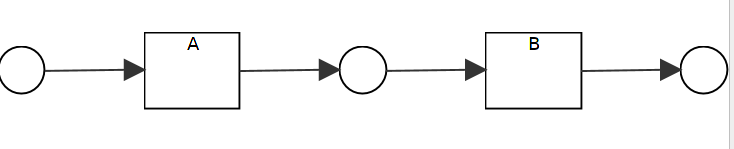
\includegraphics[width=0.9\textwidth]{figures/evaluation/model_01_sequence.png}
	\caption{Model M1 with sequence relation}
	\label{fig:sequence-M1}
\end{figure} 
\begin{itemize}
	\item \emph{Experiment 1} delete activity from sequence relation \\
	
	\emph{Event Log: }
	\begin{align*}
	Positive:& {<a>}^{50} \\
	Negative:& {<a, b>}^{50}
	\end{align*}
	% repair result from them, one is the repaired model, second is the plot lines with weight changes
	\emph{Repair Result}
	
	
	\item 
\end{itemize}
\subsubsection{Test On Parallel}
This part shows how the parallel relation of activities is affected by the weights for the existing model, positive and negative instances.

\subsubsection{Test On Loop}
This part investigated our repair method on activities with loop relation.

\subsubsection{Test On Exclusive Choice}
This part displays the changes of exclusive choices relation in the model under the different control weights.

% Conclusion part
For one exclusive choices, 
but with long-term dependency detected and added in the model, precision and accuracy increase, since model with long-term dependency blocks the negative information by adding transitions and places to limit activity selection. 
\subsection{Test On Synthetic Data}
\subsection{Test On Real life Data}